\section[Bilans énergétique et entropique]{Bilans énergétique et entropique sur un système ouvert en écoulement permanent}

    \subsection[Principes de la thermodynamique]{Formulation infinitésimale des deux principes de la thermodynamique}

        \subsubsection{Premier principe ou de \og conservation\fg~(de l'énergie)}

            \paragraph{En L1.} 
                Pour tout système fermé $\sigma$, il existe une fonction $U$, dite \og énergie interne\fg, telle que
                \begin{enumerate}
                    \item $U$ est additive (extensive). Cela implique des interactions de deux systèmes à très courte portée.
                    \item Si $\Sigma$ subit une évolution de $i\to f$, on a
                    \begin{equation*}
                        \boxed{
                            \Delta U+\Delta E_{c}^{\text{macro}}=W^{\text{ext}}+Q^{\text{ext}},
                        }
                    \end{equation*}
                    ou bien
                    \begin{equation*}
                        W^{\text{ext}}=W_{\text{cons}}^{\text{ext}}+Q^{\text{ext}}
                    \end{equation*}
                    avec $W_{\text{cons}}^{\text{ext}}=-\Delta E_p^{\text{ext}}$, d'où
                    \begin{equation*}
                        \boxed{
                            \Delta E_{\text{tot}}=W_{nc}^{\text{ext}}+Q^{\text{ext}},
                        }
                    \end{equation*}
                    où $E_{\text{tot}}=U+E_{c}^{\text{macro}}+E_p^{\text{ext}}$.
                    \item Si $\Sigma$ est à l'équilibre thermodynamique, $U$ est une fonction d'était, c'est-à-dire qu'elle est fonction d'un petit nombre de paramètres du système.
                \end{enumerate}

                \begin{remark}
                    Le plus souvent, $\Delta E_c^{\text{macro}}$ est négligeable d'où
                    \begin{equation*}
                        \boxed{
                            \Delta U=W^{\text{ext}}+Q^{\text{ext}}.
                        }
                    \end{equation*}
                \end{remark}

                \begin{remark}
                    Si on considère une transformation monobare sans autre travail que celui des forces de pression, on a $P^{\text{ext}}=\mathrm{constante}$, d'où $P_f=P_i=P^{\text{ext}}$ et 
                    \begin{equation*}
                        \delta W^{\text{ext}}=-P^{\text{ext}}\rmd V.
                    \end{equation*}
                    Ainsi,
                    \begin{align*}
                        W^{\text{ext}}
                        &=
                        W=-\int_{i}^{f}P^{\text{ext}}\rmd V,\\
                        &=
                        -P^{\text{ext}}\Delta V=-(P_f V_f-P_i V_i).
                    \end{align*}
                    On a donc 
                    \begin{equation*}
                        \Delta U=U_f-U_i=-(P_f V_f-P_i V_i)+Q^{\text{ext}}.
                    \end{equation*}
                    Donc si $H=U+PV$, on a 
                    \begin{equation*}
                        \boxed{
                            \Delta H=Q^{\text{ext}}.
                        }
                    \end{equation*}
                \end{remark}

                \begin{example}
                    Pour un gaz avec $N\sim 10^{23}$ particules, a priori $U$ est une fonction de $6N\times $ variables (positions et vitesses). Àl 'équilibre, $U$ est une fonction de la température et du volume uniquement (par exemple).
                \end{example}

            \paragraph{En L2.}

                On considère deux états infiniment proches:
                \begin{equation*}
                    \boxed{
                        \rmd U+\rmd E_c^{\text{macro}}=\delta W^{\text{ext}}+\delta Q^{\text{ext}}.
                    }
                \end{equation*}
                Le cas fréquent est $\rmd U=\delta W^{\text{ext}}+\delta Q^{\text{ext}}$.

        \subsubsection{Deuxième principe \og d'évolution\fg}

            \paragraph{En L1.}
                Pour tout système fermé $\Sigma$, il existe une fonction $S$ \og entropie\fg~telle que
                \begin{enumerate}
                    \item $S$ est additive (extensive)
                    \item Si $\Sigma$ subit une évolution de $i\to f$, alors
                    \begin{equation*}
                        \boxed{
                            \Delta S=S_{\text{créée}}+S_{\text{échangée}},
                        }
                    \end{equation*}
                    avec
                    \begin{equation*}
                        S_{\text{échangée}}=\sum_{i}\frac{Q_i^{\text{ext}}}{T_i^{\text{ext}}},\qquad S_{\text{créée}}\geqslant 0.
                    \end{equation*}
                    $T_i^{\text{ext}}$ représente l'interaction avec un thermostat. Le signe de l'entropie créée implique une évolution du système.
                    \item À l'équilibre thermodynamique, $S$ est une fonction d'état.
                \end{enumerate}

                Si le système $\Sigma$ est isolé (évolution adiabatique), on a 
                \begin{equation*}
                    \boxed{
                        S_{\text{échangée}}=0,\qquad\Delta S=S_{\text{créée}}\geqslant0.
                    }
                \end{equation*}
                Si l'évolution est réversible, on a $S_{\text{créée}}=0$, d'où 
                \begin{equation*}
                    \boxed{
                        \Delta S=S_{\text{échangée}}.
                    }
                \end{equation*}

            \paragraph{En L2.}
                On considère une transformation infinitésimale, d'où
                \begin{equation*}
                    \boxed{
                        \rmd S=\delta S_{\text{échangée}}+\delta S_{\text{créée}},\quad\delta S_{\text{créée}}\geqslant0,\quad\delta S_{\text{échangée}}=\frac{\delta Q^{\text{ext}}}{T^{\text{ext}}}.
                    }
                \end{equation*}
                Une conséquence directe est 
                \begin{equation*}
                    S_{\text{échangée}}=\int_{i}^{f}\frac{\delta Q^{\text{ext}}}{T^{\text{ext}}}.
                \end{equation*}

    \subsection{Bilan de masse pour un fluide en écoulement permanent}
        \subsubsection{Débit de masse (1D)}

            On se réfère à la Figure~\ref{fig:debit_masse_fluide_ecoulement_permanent}. Le fluide est caractérisé par une masse volumique $\mu$ supposée uniforme et constante.

            \begin{figure}
                \centering
                \tikzsetnextfilename{debit_masse_fluide_ecoulement_permanent}
                \begin{tikzpicture}[scale=1]  
                    % \helpgrid{3}{3}
    
                    \draw (-3,0)--++(6,0);
                    \draw (-3,3)--++(6,0);
                    \draw [-latex] (3.5,0)--++(0.5,0) node [right] {$x$};
                    \draw [latex-latex] (-3.5,0)--++(0,3) node [left,midway] {$S$};
                    \draw [dashed, red] (-2,0)--++(0,3);
                    \draw [dashed, pattern=north west lines, pattern color=red, draw=red] (-2,0) rectangle (-1,3);
                    \draw [-stealth, blue] (-1,0.5)--++(2,0);
                    \draw [-stealth, blue] (-1,1.5)--++(2,0);
                    \draw [-stealth, blue] (-1,2.5)--++(2,0);
                    \node at (-1,0) [below] {$x$};
                    \node at (0,0) [below] {$\vec{v}$};
                    \draw [latex-latex] (-2,3.25)--++(1,0) node [above,midway] {$v \rmd t$};
                
                \end{tikzpicture}
                \caption{Débit de masse dans un fluide en écoulement permanent.}    
                \label{fig:debit_masse_fluide_ecoulement_permanent}
            \end{figure}

            Une quantité de masse $\delta m$ du fluide traverse une section $S$ pendant une période de temps $\rmd t$. Ainsi,
            \begin{equation*}
                \delta m=(S\times v\rmd t)\times\mu=\mu v S\rmd t.
            \end{equation*}
            On pose alors 
            \begin{equation*}
                \boxed{
                    D_m=\frac{\delta m}{\rmd t}=\mu v S.
                }
            \end{equation*}
            C'est la quantité de masse traversant une section $S$ par unité de temps. Notons que [$\mu$]=\si[]{\kilogram\per\metre\cubed}, [$v$]=\si[]{\metre\per\second} et [$S$]=\si[]{\metre\squared}.

        \subsubsection{Bilan de masse en régime permanent}

            \paragraph{Une entrée, une sortie.}

                On est en écoulement permanent et on considère un système ouvert $\Sigma(t)$ et $V$ est un volume de contrôle (fixe), voir la Figure~\ref{fig:bilan_masse_regime_permanent_une_entree_une_sortie}.

                \begin{figure}
                    \centering
                    \tikzsetnextfilename{bilan_masse_regime_permanent_une_entree_une_sortie}
                    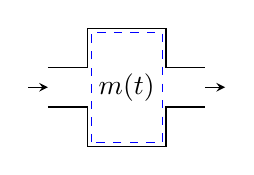
\begin{tikzpicture}[scale=1]  
                        % \helpgrid{3}{3}
        
                        \draw (-1,0)--++(0.5,0)--++(0,0.5)--++(1,0)--++(0,-0.5)--++(0.5,0);
                        \draw (-1,-0.5)--++(0.5,0)--++(0,-0.5)--++(1,0)--++(0,0.5)--++(0.5,0);
                        \draw [draw=blue, dashed] (-0.45,-0.95) rectangle (0.45,0.45);                 
                        \node at (0.,-0.25) {$m(t)$};
                        \draw [-stealth] (-1.25,-0.25)--++(0.25,0);
                        \draw [-stealth] (1,-0.25)--++(0.25,0);
                    \end{tikzpicture}
                    \caption{Bilan de masse en régime permanent, une entrée et une sortie.}    
                    \label{fig:bilan_masse_regime_permanent_une_entree_une_sortie}
                \end{figure}

                Il faut définir un système fermé $\Sigma^{\star}$ (donc de masse constante $m^{\star}$). On considère donc la Figure~\ref{fig:bilan_masse_regime_permanent_une_entree_une_sortie_systeme_ferme}.

                \begin{figure}
                    \centering
                    \tikzsetnextfilename{bilan_masse_regime_permanent_une_entree_une_sortie_systeme_ferme}
                    \begin{tikzpicture}[scale=1]  
                        % \helpgrid{3}{3}
        
                        \draw (-1,0)--++(0.5,0)--++(0,0.5)--++(1,0)--++(0,-0.5)--++(0.5,0);
                        \draw (-1,-0.5)--++(0.5,0)--++(0,-0.5)--++(1,0)--++(0,0.5)--++(0.5,0);
                        \draw [draw=red, dashed] (-1,-0.05)--++(0.55,0)--++(0,0.49)--++(0.9,0)--++(0,-1.4)--++(-0.9,0)--++(0,0.5)--++(-0.5,0)--++(0,0.4);
                        \draw [dashed, draw=green,pattern=north west lines, pattern color=green] (-1,-0.5) rectangle (-0.5,0);
                        \node [text=red] at (0.,-0.25) {$\Sigma (t)$};
                        \node [text=green] at (-1,0.25) {$\delta m_e$};
                        \node at (0,1) {à $t$};

                        \draw (3,0)--++(0.5,0)--++(0,0.5)--++(1,0)--++(0,-0.5)--++(0.5,0);
                        \draw (3,-0.5)--++(0.5,0)--++(0,-0.5)--++(1,0)--++(0,0.5)--++(0.5,0);
                        \draw [draw=red, dashed] (3.55,0.45)--++(0.9,0)--++(0,-0.5)--++(0.5,0)--++(0,-0.4)--++(-0.5,0)--++(0,-0.5)--++(-0.95,0)--++(0,1.4);
                        \draw [dashed, draw=green,pattern=north west lines, pattern color=green] (4.5,-0.5) rectangle (5,0);
                        \node [text=red] at (4,-0.25) {\tiny$\Sigma (t+\rmd t)$};
                        \node [text=green] at (5.2,0.25) {$\delta m_s$};
                        \node at (4,1) {à $t+\rmd t$};
                    \end{tikzpicture}
                    \caption{Bilan de masse en régime permanent, une entrée et une sortie, système fermé.}    
                    \label{fig:bilan_masse_regime_permanent_une_entree_une_sortie_systeme_ferme}
                \end{figure}

                $\sigma^{\star}$ est fermé, on a $m^{\star}(t)=m^{\star}(t+\rmd t)$ d'où
                \begin{equation*}
                    m(t)+\delta m_e=m(t+\rmd t)+\delta m_s=m(t)+D_m^{e}\rmd t=m(t+\rmd t)+D_m^{s}\rmd t.
                \end{equation*}
                En régime permanent, on a $m(t+\rmd t)=m(t)$, donc 
                \begin{equation*}
                    \boxed{
                        D_m^{e}=D_{m}^{s}.
                    }
                \end{equation*}

            \paragraph{Plusieurs entrées, plusieurs sorties.}

                On considère le système présenté à la Figure~\ref{fig:bilan_masse_regime_permanent_plusieurs_entrees_plusieurs_sorties}.

                \begin{figure}
                    \centering
                    \tikzsetnextfilename{bilan_masse_regime_permanent_plusieurs_entrees_plusieurs_sorties}
                    \begin{tikzpicture}[scale=1]  
                        % \helpgrid{3}{3}
        
                        \draw (0,0)--(1,0)--(1,1)--(3,1)--(3,-0.5)--(4,-0.5);
                        \draw (0,-0.5)--(1,-0.5)--(1,-1)--(0,-1);
                        \draw (0,-1.5)--(1,-1.5)--(1,-2)--(0,-2);
                        \draw (0,-2.5)--(1,-2.5)--(1,-3.5)--(3,-3.5)--(3,-2)--(4,-2);
                        \draw (4,-1)--(3,-1)--(3,-1.5)--(4,-1.5);
                        \draw [-stealth] (-0.5,-0.25)--++(0.5,0) node [left,pos=0] {1};
                        \draw [-stealth] (-0.5,-1.25)--++(0.5,0) node [,left,pos=0] {2};
                        \draw [-stealth] (-0.5,-2.25)--++(0.5,0) node [left,pos=0] {3};
                        \draw [-stealth] (4,-0.75)--++(0.5,0) node [right,pos=1] {1'};
                        \draw [-stealth] (4,-1.75)--++(0.5,0) node [right,pos=1] {2'};
                        \draw [dashed, draw=blue] (1.05,-3.45) rectangle (2.95,0.95);
                        \node [text=blue] at (2,-1) {$\Sigma (t)$};
                    \end{tikzpicture}
                    \caption{Bilan de masse en régime permanent, plusieurs entrées et plusieurs sorties.}    
                    \label{fig:bilan_masse_regime_permanent_plusieurs_entrees_plusieurs_sorties}
                \end{figure}

                En régime permanent le même raisonnement amène à
                \begin{equation*}
                    \boxed{
                        \sum_{i}D_{m_i}^{e}=\sum_{j}D_{m_j}^{s}.
                    }
                \end{equation*}
    
    \subsection{Bilan énergétique en régime permanent}

        On considère le système présenté à la Figure~\ref{fig:bilan_energetique_regime_permanent_systeme_ouvert}. Les entrées sont $u_e,v_e$ et $P_e$. Les sorties sont $u_s,v_s,P_s$. Comme précédemment, on note $\Sigma^{\star}(t)$ le système fermé considéré au temps $t$, et $\Sigma^{\star}(t+\rmd t)$ le système fermé considéré au temps $t+\rmd t$. Les flèches autour du système indique les forces de pression.

        \begin{figure}
            \centering
            \tikzsetnextfilename{bilan_energetique_regime_permanent_systeme_ouvert}
            \begin{tikzpicture}[scale=1]  
                % \helpgrid{3}{3}

                \draw (-1,0)--(0,0)--(4,0)--(4,3)--(5,3)--(5,4)--(4,4)--(0,4)--(0,1)--(-1,1)--(-1,0);
                \draw [draw=red, dashed] (-1,0)--(4,0)--(4,4)--(0,4)--(0,1)--(-1,1)--(-1,0);
                \draw [draw=green,dashed] (0,0)--(4,0)--(4,3)--(5,3)--(5,4)--(0,4)--(0,0);
                \node at (2,2) {\Huge$\star$};
                \draw [->] (2,2.5) to[bend right=45] (1.5,2);
                \node [text=red] at (-1.5,2) {$\Sigma^{\star}(t)$};
                \node [text=green] at (5.5,1) {$\Sigma^{\star}(t+\rmd t)$};
                \node at (2,5) {$\Sigma(t)$};
                \draw [-stealth] (-2.5,-1)--(-2.5,5);
                \node at (-2.5,0.5) {$\bullet$};
                \node at (-2.5,3.5) {$\bullet$};
                \node at (-2.5,0.5) [left] {$z_e$};
                \node at (-2.5,3.5) [left] {$z_s$};
                \draw [-stealth] (6.5,4)--++(0,-2) node [left, midway] {$\vec{g}$};
                \draw [->] (-1.5,0.5)--++(0.5,0) node [below left] {$D_m$};
                \draw [->] (5,3.5)--++(0.5,0) node [above] {$D_m$};
                \draw [->] (0.5,-0.5)--++(0,0.5);
                \draw [->] (1.5,-0.5)--++(0,0.5);
                \draw [->] (2.5,-0.5)--++(0,0.5);
                \draw [->] (3.5,-0.5)--++(0,0.5);
                \draw [->] (-0.5,1.5)--++(0.5,0);
                \draw [->] (-0.5,2.5)--++(0.5,0);
                \draw [->] (-0.5,3.5)--++(0.5,0);
                \draw [->] (0.5,4.5)--++(0,-0.5);
                \draw [->] (1.5,4.5)--++(0,-0.5);
                \draw [->] (2.5,4.5)--++(0,-0.5);
                \draw [->] (3.5,4.5)--++(0,-0.5);
                \draw [->] (4.5,2.5)--++(-0.5,0);
                \draw [->] (4.5,1.5)--++(-0.5,0);
                \draw [->] (4.5,0.5)--++(-0.5,0);
            \end{tikzpicture}
            \caption{Bilan d'énergie en régime permanent.}    
            \label{fig:bilan_energetique_regime_permanent_systeme_ouvert}
        \end{figure}

        \subsubsection{Bilan énergétique}

            On définit $E\coloneqq U+E_c^{\text{macro}}+E_p^{\text{pes}}$. $\Sigma^{\star}$ étant fermé, on a 
            \begin{align*}
                E^{\star}(t)
                &=E(t)+\delta E_e=E(t)+\delta m_e\left[u_e+\frac{v_e^{2}}{2}+gz_e\right],\\
                &=E^{\star}(t+\rmd t),\\
                &= E(t+\rmd t)+\delta E_s=E(t+\rmd t)+\delta m_s\left[u_s+\frac{v_s^{2}}{2}+g z_s\right].
            \end{align*}
            En régime permanent, on a $E(t+\rmd t)=E(t)$ et $\delta m_e=\delta m_s=D_m\rmd t$, d'où
            \begin{equation*}
                \boxed{
                    \frac{\rmd E^{\star}}{\rmd t}=D_m\left[\left(u_s+\frac{v_s^{2}}{2}+g z_s\right)-\left(u_e+\frac{v_e^{2}}{2}+g z_e\right)\right].
                }
            \end{equation*}

        \subsubsection{Premier principe}

            On a 
            \begin{equation*}
                \frac{\rmd E^{\star}}{\rmd t}=\frac{\delta W_{\text{nc}}^{\text{ext}}}{\rmd t}+\frac{\delta Q^{\text{ext}}}{\rmd t}=P_{\text{méca,nc}^{\text{ext}}}+P_{\text{th}}^{\text{ext}}.
            \end{equation*}
            Notamment, 
            \begin{equation*}
                P_{\text{méca,nc}}^{\text{ext}}=P_{\text{press}}^{\text{ext}}+P_{\text{indiquées}},
            \end{equation*}
            où le deuxième terme vient des échanges avec les parties mobiles. Comme $D_m=\mu SV$, on a 
            \begin{align*}
                P_{\text{press}}^{\text{ext}}
                &=Pe S_e\vec{u_x}\cdot v_e\vec{u_x}+(-P_s S_s\vec{u_x})\cdot v_s\vec{u_x},\\
                &=P_e S_e V_e-P_s S_s V_s = D_m\left[\frac{P_e}{\mu_e}-\frac{P_s}{\mu_s}\right].
            \end{align*}

            Donc
            \begin{equation*}
                D_m\left[\left(u_s+\frac{v_s^{2}}{2}+g z_s+\frac{P_s}{\mu_s}\right)-\left[u_e+\frac{v_e^{2}}{2}+g z_e+\frac{P_e}{\mu_e}\right]\right]=P_i+P_{\text{th}}^{\text{ext}}.
            \end{equation*}
            En notant $H=U+PV$, et $h=u+Pv_m$ où $v_m=\frac{1}{\mu}$, on a
            \begin{equation*}
                \boxed{
                    D_m\left[\left(h_s+\frac{v_s^{2}}{2}+g z_s\right)-\left(h_e+\frac{v_e^{2}}{2}+g z_e\right)\right]=P_i+P_{\text{th}}^{\text{ext}}.
                }
            \end{equation*}

            En formulation intensive, on note le travail indiqué massique
            \begin{equation*}
                \boxed{
                    \frac{P_i}{D_m}\coloneqq\omega_i,
                }
            \end{equation*}
            d'unité \si[]{\watt\second\per\kilogram}. On note le transfert thermique massique 
            \begin{equation*}
                \boxed{
                    \frac{P_{\text{th}}}{D_m}\coloneqq q.
                }
            \end{equation*}
            Alors
            \begin{equation*}
                \left(h_s+\frac{v_s^{2}}{2}+g z_s\right)-\left[h_e+\frac{v_e^{2}}{2}+g z_e\right]=\omega_i+q.
            \end{equation*}

    \subsection{Bilan entropique en régime permanent}
        
        \subsubsection{Bilan entropique}
            
            On considère toujours le système présenté à la Figure~\ref{fig:bilan_energetique_regime_permanent_systeme_ouvert}. On a 
            \begin{equation*}
                \begin{aligned}
                    S^{\star}(t)&= S(t)+\delta S_e=S(t)+\delta m_e s_e,\\
                    S^{\star}(t+\rmd t)&= S(t+\rmd t)+\delta m_s s_s.
                \end{aligned}
            \end{equation*}
            En régime permanent, on a donc
            \begin{equation*}
                \boxed{
                    \frac{\rmd S^{\star}}{\rmd t}=D_m\left(S_s-S_e\right).
                }
            \end{equation*}

        \subsubsection{Second principe}
            
            On a 
            \begin{equation*}
                \frac{\rmd S^{\star}}{\rmd t}=\frac{\delta S_{\text{ech}}}{\rmd t}+\frac{\delta S_{\text{cr}}}{\rmd t},
            \end{equation*}
            où le deuxième terme est positif. Ainsi,
            \begin{equation*}
                \boxed{
                    D_m\left[S_s-S_e\right]=\frac{\delta S_{\text{ech}}}{\rmd t}+\frac{\delta S_{\text{cr}}}{\rmd t}.
                }
            \end{equation*}
            En formulation intensive, on note l'entropie échangée par unité de masse
            \begin{equation*}
                \boxed{
                    \frac{1}{D_m}\frac{\delta S_{\text{ech}}}{\rmd t}=s_{\text{ech}}.
                }
            \end{equation*}
            L'entropie créée par unité de masse est donnée par
            \begin{equation*}
                \boxed{
                    \frac{1}{D_m}\frac{\delta S_{\text{cr}}}{\rmd t}=s_{\text{cr}}.
                }
            \end{equation*}

            En régime permanent, on a donc
            \begin{equation*}
                \boxed{s_s-s_e=s_{\text{ech}}+s_{\text{cr}}}.
            \end{equation*}

            Dans le cas monotherme, on a
            \begin{equation*}
                \frac{\delta S_{\text{ech}}}{\rmd t}=\frac{P_{\text{th}}^{\text{ext}}}{T^{\text{ext}}},
            \end{equation*}
            et
            \begin{equation*}
                \boxed{
                    s_{\text{ech}}=\frac{q}{T^{\text{ext}}}.
                }
            \end{equation*}
            Finalement, en régime permanent et dans le cas monotherme, on a
            \begin{equation*}
                \boxed{
                    s_s-s_e=\frac{q}{T^{\text{ext}}}+s_c.
                }
            \end{equation*}
            Dans le cas adiabatique, on a
            \begin{equation*}
                \boxed{
                    s_s-s_e=s_c\geqslant 0.
                }
            \end{equation*}

    \subsection{Exemples}
        \subsubsection{Détente de Joule-Kelvin/Joule-Thompson}

            C'est un écoulement adiabatique, lent et permanent, considéré à la Figure~\ref{fig:detente_joule_kelvin}, où l'on a $P_e>P_s$.

            \begin{figure}
                \centering
                \tikzsetnextfilename{detente_joule_kelvin}
                \begin{tikzpicture}[scale=1]  
                    % \helpgrid{3}{3}
    
                    \draw [pattern=north west lines] (-3,-0.5) rectangle (3,0);
                    \draw [pattern=north west lines] (-3,2) rectangle (3,2.5);
                    \draw (-1,0)--(0,0.75)--(1,0);
                    \draw (-1,2)--(0,1.25)--(1,2);
                    \draw [->] (-2,1)--++(1,0) node [above, midway] {$P_e$};
                    \draw [->] (1.5,1)--++(1,0) node [above, midway] {$P_s$};
                \end{tikzpicture}
                \caption{Détente de Joule-Kelvin.}    
                \label{fig:detente_joule_kelvin}
            \end{figure}

            Dans le bilan énergétique, on considère que les vitesses sont lentes (donc négligeables dans le bilan) et que la variation de hauteur est de l'ordre d'une dizaine de centimètres (négligeable dans le bilan). Ainsi,
            \begin{equation*}
                h_s-h_s=\omega_i+q=0,
            \end{equation*}
            car il n'y a pas de transferts thermique ni de travail. Finalement, on a 
            \begin{equation*}
                \boxed{
                    h_s=h_e,\quad s_s>s_e.
                }
            \end{equation*}

        \subsubsection{Compresseur/Turbine}

            Dans un compresseur, il y a une augmentation de la pression du fluide en lui fournissant du travail $\omega_i>0$. Dans une turbine, le fluide entraîne la turbine donc $\omega_i<0$. On modélise ces deux systèmes par la Figure~\ref{fig:compresseur_turbine}.

            \begin{figure}
                \centering
                \tikzsetnextfilename{compresseur_turbine}
                \begin{tikzpicture}[scale=1]  
                    % \helpgrid{3}{3}
    
                    \draw (-2,1)--(0,1);
                    \draw (-2,0)--(0,0);
                    \draw[pattern=grid] (0.5,0.5) circle (0.707);
                    \draw (1,1)--(3,1);
                    \draw (1,0)--(3,0);
                    \draw [->] (-1.5,0.5)--++(1,0) node [above,midway] {$e$};
                    \draw [->] (1.5,0.5)--++(1,0) node [above,midway] {$s$};
                    \node at (0.5,1.5) {Compresseur ou Turbine};
                \end{tikzpicture}
                \caption{Compresseur ou turbine.}    
                \label{fig:compresseur_turbine}
            \end{figure}

            À nouveau, en négligeant les vitesses et la variation de hauteur, et en supposant que les transferts thermiques sont négligeables, on a 
            \begin{equation*}
                \boxed{
                    \Delta h=\omega_i,\quad \Delta s\gtrapprox0.
                }
            \end{equation*}

        \subsubsection{Tuyère}
            On considère une tuyère à la Figure~\ref{fig:tuyere}. La vitesse augment du gaz augmente de gauche à droite, $c_s$ est la vitesse du son.. L'écoulement est rapide, il n'y a pas de parties mobiles ($\omega_i=0$) et il n'y a pas le temps pour qu'il y ait des transferts thermiques (évolution adiabatique, $q\approx0$).

            Ainsi,
            \begin{equation*}
                \Delta h+\Delta\left(\frac{v^{2}}{2}\right)=0.
            \end{equation*}
            Pour $v_s\gg v_e$, on a
            \begin{align*}
                \dfrac{v_s^{2}}{2}
                &\approx-\Delta h,\\
                &=-C_{p,m}\Delta T,\\
                &=-\frac{\gamma r}{\left(\gamma-1\right)M}\Delta T>0,
            \end{align*}
            où l'on a utilisé la loi des gaz parfaits et l'on a noté $\gamma=\dfrac{C_p}{C_V}$. Ainsi, $\Delta T<0$.

            \begin{figure}
                \centering
                \tikzsetnextfilename{tuyere}
                \begin{tikzpicture}[scale=1]  
                    % \helpgrid{3}{3}
    
                    \draw[pattern=north east lines] (0,0) arc(0:180:5 and 1);
                    \draw[pattern=north east lines] (0,3) arc(0:-180:5 and 1);
                    \draw [dashed] (-5,3.5)--(-5,-0.5) node [below] {$\frac{v}{c_s}=1$};
                    \node at (-7.5, -0.75) {$\frac{v}{c_s}<1$};
                    \node at (-2.5, -0.75) {$\frac{v}{c_s}>1$};
                    \draw[->] (-8,1.5)--++(1,0) node [above, midway] {$\vec{v}$};
                    \draw[->] (-4,1.5)--++(2.5,0) node [above, midway] {$\vec{v}$};
                \end{tikzpicture}
                \caption{Tuyère.}    
                \label{fig:tuyere}
            \end{figure}
            




